\title{\~Study Notes}
\date{Last updated on : \today}

\documentclass[12pt]{article}
%\usepackage{hyperref}% http://ctan.org/pkg/hyperref
%\usepackage{bookmark}% http://ctan.org/pkg/bookmark
\usepackage[bookmarks,bookmarksopen,bookmarksdepth=9]{hyperref}
\usepackage{scrextend}	% For margin
\usepackage{xcolor}	% For colors
\usepackage{tikz} % For tree
\usepackage{tikz-qtree}
\usepackage{msc}
\usepackage{graphicx}
\usepackage{multicol}

\begin{document}
\maketitle
\pagebreak

%\begin{abstract}
%This is the paper's abstract \ldots
%\end{abstract}
\tableofcontents





%%%%%%%%%%%%%%%%%%%%%%%%%%%%%%%%%%%%%%%%%%%%%%%%%%%%%%%%%%%%%%%%%%%%%
%
%	Description of this section
%
%%%%%%%%%%%%%%%%%%%%%%%%%%%%%%%%%%%%%%%%%%%%%%%%%%%%%%%%%%%%%%%%%%%%%
%\pagebreak
%\vspace*{\fill}
%\begin{center}
%\section{Section Title}
%Description of this section
%\end{center}
%\vspace*{\fill}
%\pagebreak







%%%%%%%%%%%%%%%%%%%%%%%%%%%%%%%%%%%%%%%%%%%%%%%%%%%%%%%%%%%%%%%%%%%%%
%
%	Figures of Speech
%
%%%%%%%%%%%%%%%%%%%%%%%%%%%%%%%%%%%%%%%%%%%%%%%%%%%%%%%%%%%%%%%%%%%%%
\pagebreak
\vspace*{\fill}
\begin{center}
\section{Figures of Speech}
Figures of Speech
\end{center}
\vspace*{\fill}
\pagebreak

\subsection{Uses}
\begin{itemize}
\item Ornamental 
\item Clearness
\end{itemize}

\subsection{Types}
\begin{itemize}
\item Similarity
\begin{multicols}{3}
\begin{itemize}
\item Simile
\item Metaphor
\item Allegory
\item Fable
\item Parable
\item Personification
\end{itemize}
\end{multicols}

\item Contrast
\begin{multicols}{3}
\begin{itemize}
\item Antithesis
\item Oxymoron 
\item Epigram
\item Irony
\item Sarcasm
\item Innuendo
\item Hyperbole
\item Litotes 
\item Euphemism 
\item Pun
\end{itemize}
\end{multicols}

\item Association
\begin{multicols}{3}
\begin{itemize}
\item Metonymy 
\item Synecdoche
\end{itemize}
\end{multicols}

\item Arrangement
\begin{multicols}{3}
\begin{itemize}
\item Interrogation  
\item Apostrophe  
\item Repetition  
\item Pleonasm  
\item Bathos [Anticlimax]
\item Climax
\end{itemize}
\end{multicols}
\end{itemize}

%%%%%%%%%%%%%%%%%%%%%%%%%%%%%%%%%%%%%%%%%%%%%%%%%%%%%%%%%%%%%%%%%%%%%
%
%	Classification of Mamals
%
%%%%%%%%%%%%%%%%%%%%%%%%%%%%%%%%%%%%%%%%%%%%%%%%%%%%%%%%%%%%%%%%%%%%%
\pagebreak
\vspace*{\fill}
\begin{center}
\section{Classification of Mammals }
This section documents how the mammals are classified based on the 
reproductive technique.
\end{center}
\vspace*{\fill}
\pagebreak

\subsection{Types of Mammals}
\begin{center}
\Tree [.Mammals [.Egg\ laying(Monotremes) ] [.Giving\ Birth(therians) [.Pouched(marsupials) ] [.Placental(eutherians) ] ]]
\end{center}



%%%%%%%%%%%%%%%%%%%%%%%%%%%%%%%%%%%%%%%%%%%%%%%%%%%%%%%%%%%%%%%%%%%%%
%
%	Cryptanalysis and Attacks on Cryptosystems 
%
%%%%%%%%%%%%%%%%%%%%%%%%%%%%%%%%%%%%%%%%%%%%%%%%%%%%%%%%%%%%%%%%%%%%%
\pagebreak
\vspace*{\fill}
\begin{center}
\section{Cryptanalysis and Attacks on Cryptosystems }
This section is study notes on Cryptanalysis and Attacks on Cryptosystems 
Reference : 	\url {http://math.colorado.edu/~hiba/crypto/cryptanalysis.html}
\end{center}
\vspace*{\fill}
\pagebreak

Cryptanalysis is the art of deciphering encrypted communications without knowing the proper keys. There are many cryptanalytic techniques. Some of the more important ones for a system implementer are described below.

\subsection{Ciphertext-only attack}
This is the situation where the attacker does not know anything about the contents of the message, and must work from ciphertext only. In practice it is quite often possible to make guesses about the plaintext, as many types of messages have fixed format headers. Even ordinary letters and documents begin in a very predictable way. For example, many classical attacks use frequency analysis of the ciphertext, however, this does not work well against modern ciphers.

Modern cryptosystems are not weak against ciphertext-only attacks, although sometimes they are considered with the added assumption that the message contains some statistical bias.

\subsection{Known-plaintext attack}
The attacker knows or can guess the plaintext for some parts of the ciphertext. The task is to decrypt the rest of the ciphertext blocks using this information. This may be done by determining the key used to encrypt the data, or via some shortcut.

One of the best known modern known-plaintext attacks is linear cryptanalysis against block ciphers.

\subsection{Chosen-plaintext attack}
The attacker is able to have any text he likes encrypted with the unknown key. The task is to determine the key used for encryption.

A good example of this attack is the differential cryptanalysis which can be applied against block ciphers (and in some cases also against hash functions).

Some cryptosystems, particularly RSA, are vulnerable to chosen-plaintext attacks. When such algorithms are used, care must be taken to design the application (or protocol) so that an attacker can never have
chosen plaintext encrypted.

\subsection{Man-in-the-middle attack}
This attack is relevant for cryptographic communication and key exchange
protocols. The idea is that when two parties, A and B, are exchanging keys for secure communication (e.g., using Diffie-Hellman), an adversary positions himself between A and B on the communication line. The adversary then intercepts the signals that A and B send to each other, and performs a key exchange with A and B separately. A and B will end up using a different key, each of which is known to the adversary. The adversary can then decrypt any communication from A with the key he shares with A, and then resends the communication to B by encrypting it again with the key he shares with B. Both A and B will think that they are communicating securely, but in fact the adversary is hearing everything.

The usual way to prevent the man-in-the-middle attack is to use a public key cryptosystem capable of providing digital signatures. For set up, the parties must know each others public keys in advance. After the shared secret has been generated, the parties send digital signatures of it to each other. The man-in-the-middle can attempt to forge these signatures, but fails because he cannot fake the signatures.

This solution is sufficient in the presence of a way to securely distribute public keys. One such way is a certificate hierarchy such as X.509. It is used for example in IPSec.

Correlation between the secret key and the output of the cryptosystem is the main source of information to the cryptanalyst. In the easiest case, the information about the secret key is directly leaked by the cryptosystem. More complicated cases require studying the correlation (basically, any relation that would not be expected on the basis of chance alone) between the observed (or measured) information about the cryptosystem and the guessed key information.

For example, in linear (resp. differential) attacks against block ciphers the cryptanalyst studies the known (resp. chosen) plaintext and the observed ciphertext. Guessing some of the key bits of the cryptosystem the analyst determines by correlation between the plaintext and the ciphertext whether she guessed correctly. This can be repeated, and has many variations.

The differential cryptanalysis introduced by Eli Biham and Adi Shamir in late 1980's was the first attack that fully utilized this idea against block ciphers (especially against DES). Later Mitsuru Matsui came up with linear cryptanalysis which was even more effective against DES. More recently, new attacks using similar ideas have been developed.

Perhaps the best introduction to this material is the proceedings of EUROCRYPT and CRYPTO throughout the 1990's. There can be found Mitsuru Matsui's discussion of linear cryptanalysis of DES, and the ideas of truncated differentials by Lars Knudsen (for example, IDEA cryptanalysis). The book by Eli Biham and Adi Shamir about the differential cryptanalysis of DES is the "classical" work on this subject.

The correlation idea is fundamental to cryptography and several researchers have tried to construct cryptosystems which are provably secure against such attacks. For example, Knudsen and Nyberg have studied provable security against differential cryptanalysis.

Attack against or using the underlying hardware: in the last few years as more and more small mobile crypto devices have come into widespread use, a new category of attacks has become relevant which aim directly at the hardware implementation of the cryptosystem.

The attacks use the data from very fine measurements of the crypto device doing, say, encryption and compute key information from these measurements. The basic ideas are then closely related to those in other correlation attacks. For instance, the attacker guesses some key bits and attempts to verify the correctness of the guess by studying correlation against her measurements.

Several attacks have been proposed such as using careful timings of the device, fine measurements of the power consumption, and radiation patterns. These measurements can be used to obtain the secret key or other kinds information stored on the device.

This attack is generally independent of the used cryptographical algorithms and can be applied to any device that is not explicitly protected against it.

Faults in cryptosystems can lead to cryptanalysis and even the discovery of the secret key. The interest in
cryptographical devices lead to the discovery that some algorithms behaved very badly with the introduction of small faults in the internal computation.

For example, the usual implementation of RSA private key operations are very susceptible to fault attacks. It has been shown that by causing one bit of error at a suitable point can reveal the factorization of the modulus (i.e. it reveals the private key).

Similar ideas have been applied to a wide range of algorithms and devices. It is thus necessary that cryptographical devices are designed to be highly resistant against faults (and against malicious introduction of faults by cryptanalysts).

\subsection{Quantum computing}
Peter Shor's paper on polynomial time factoring and discrete logarithm algorithms
with quantum computers has caused growing interest in quantum computing. Quantum computing is a recent field of research that uses quantum mechanics to build computers that are, in theory, more powerful than modern serial computers. The power is derived from the inherent parallelism of quantum mechanics. So instead of doing tasks one at a time, as serial machines do, quantum computers can perform them all at once. Thus it is hoped that with
quantum computers we can solve problems infeasible with serial machines.

Shor's results imply that if quantum computers could be implemented effectively then most of public key cryptography will become history. However, they are much less effective against secret key cryptography.

Current state of the art of quantum computing does not appear alarming, as only very small machines have been implemented. The theory of quantum computation gives much promise for better performance than serial computers, however, whether it will be realized in practice is an open question.

Quantum mechanics is also a source for new ways of data hiding and secure communication with the potential of offering unbreakable security, this is the field of quantum cryptography. Unlike quantum computing, many successful experimental implementations of quantum cryptography have been already achieved. However, quantum cryptography is still some way off from being realized in commercial applications.

\subsection{DNA cryptography}
Leonard Adleman (one of the inventors of RSA) came up with the idea of using DNA as
computers. DNA molecules could be viewed as a very large computer capable of parallel execution. This parallel nature could give DNA computers exponential speed-up against modern serial computers.

There are unfortunately problems with DNA computers, one being that the exponential speed-up requires also exponential growth in the volume of the material needed. Thus in practice DNA computers would have limits
on their performance. Also, it is not very easy to build one.














%%%%%%%%%%%%%%%%%%%%%%%%%%%%%%%%%%%%%%%%%%%%%%%%%%%%%%%%%%%%%%%%%%%%%
%
%	Strength of Cryptographic Algorithms
%
%%%%%%%%%%%%%%%%%%%%%%%%%%%%%%%%%%%%%%%%%%%%%%%%%%%%%%%%%%%%%%%%%%%%%
\pagebreak
\vspace*{\fill}
\begin{center}
\section{Strength of Cryptographic Algorithms }
This section is study notes on Strength of Cryptographic Algorithms 
Reference : 	\url {http://math.colorado.edu/~hiba/crypto/strength.html}
\end{center}
\vspace*{\fill}
\pagebreak




Good cryptographic systems should always be designed so that they are as difficult to break as possible. It is possible to build systems that cannot be broken in practice (though this cannot usually be proved). This does not significantly increase system implementation effort; however, some care and expertise is required. There is no excuse for a system designer to leave the system breakable. Any mechanisms that can be used to circumvent security must be made explicit, documented, and brought into the attention of the end users.

In theory, any cryptographic method with a key can be broken by trying all possible keys in sequence. If using brute force to try all keys is the only option, the required computing power increases exponentially with the length of the key. A 32 bit key takes 232 (about 109) steps. This is something anyone can do on his/her home computer. A system with 40 bit keys takes 240 steps - this kind of computation requires something like a week (depending on the efficiency of the algorithm) on a modern home computer. A system with 56 bit keys (such as DES) takes a substantial effort (with a large number of home computers using distributed effort, it has been shown to take just a few months), but is easily breakable with special hardware. The cost of the special hardware is substantial but easily within reach of organized criminals, major companies, and governments. Keys with 64 bits are probably breakable now by major governments, and within reach of organized criminals, major companies, and lesser governments in few years. Keys with 80 bits appear good for a few years, and keys with 128 bits will probably remain unbreakable by brute force for the foreseeable future. Even larger keys are sometimes used.

However, key length is not the only relevant issue. Many ciphers can be broken without trying all possible keys. In general, it is very difficult to design ciphers that could not be broken more effectively using other methods. Designing your own ciphers may be fun, but it is not recommended for real applications unless you are a true expert and know exactly what you are doing.

One should generally be very wary of unpublished or secret algorithms. Quite often the designer is then not sure of the security of the algorithm, or its security depends on the secrecy of the algorithm. Generally, no algorithm that depends on the secrecy of the algorithm is secure. Particularly in software, anyone can hire someone to disassemble and reverse-engineer the algorithm. Experience has shown that the vast majority of secret algorithms that have become
public knowledge later have been pitifully weak in reality.

The key lengths used in public-key cryptography are usually much longer than those used in symmetric ciphers. This is caused by the extra structure that is available to the cryptanalyst. There the problem is not that of guessing the right key, but deriving the matching secret key from the public key. In the case of RSA, this could be done by factoring a large integer that has two large prime factors. In the case of some other cryptosystems it is equivalent to computing the discrete logarithm modulo a large integer (which is believed to be roughly comparable to factoring when the moduli is a large prime number). There are public key cryptosystems based on yet other problems.

To give some idea of the complexity for the RSA cryptosystem, a 256 bit modulus is easily factored at home, and 512 bit keys can be broken by university research groups within a few months. Keys with 768 bits are probably not secure in the long term. Keys with 1024 bits and more should be safe for now unless major cryptographical advances are made against RSA; keys of 2048 bits are considered by many to be secure for decades.

It should be emphasized that the strength of a cryptographic system is usually equal to its weakest link. No aspect of the system design should be overlooked, from the choice algorithms to the key distribution and usage policies.











%%%%%%%%%%%%%%%%%%%%%%%%%%%%%%%%%%%%%%%%%%%%%%%%%%%%%%%%%%%%%%%%%%%%%
%
%	Diffie Hellman Scheme
%
%%%%%%%%%%%%%%%%%%%%%%%%%%%%%%%%%%%%%%%%%%%%%%%%%%%%%%%%%%%%%%%%%%%%%
\pagebreak
\vspace*{\fill}
\begin{center}
\section{Diffie Hellman Scheme}
This section is study notes on Diffie Hellman Computational assumption, Decisive assumption 
and Key Exchange protocol.
\end{center}
\vspace*{\fill}
\pagebreak
The \textbf{Diffie-Hellman assumption's} are the assumption's that a certain 
computational problem within a cyclic group is hard.
\subsection{Computational Diffie-Hellman assumption}
\begin{itemize}
\item The CDH assumption is related to the \textit{\textbf{discrete logarithm assumption}}.
\item Given $(g,g^a,g^b) \,$ its hard to compute $g^{ab}$
\end{itemize}

\subsection{Decisional Diffie-Hellman assumption}
\begin{itemize}
\item Chosen $a,b \in Z_p$, Given $(g,a,b,g^a,g^b,) \,$ and  the value $g^{ab}$ "looks like" a  random element in G
\end{itemize}

\subsection{Diffie Hellman Key Exchange}
\begin{itemize}
\item Generate tow prime numbers $(g,p)$
\item Communicate $(g,p)$ and consider its available with both \textit{Alice} and \textit{Bob}

\item Alice picks a random secret, $a$ and computes
\begin{itemize}
\item $A$ = $g^a \bmod p$
\end{itemize}

\item Bob picks a random secret, $b$ and computes
\begin{itemize}
\item $B$ = $g^b \bmod p$
\end{itemize}

\item Alice and Bob exchange $A$ and $B$

\item Alice Computes, $A'$ as following
\begin{itemize}
\item $A'$ = $B^a \bmod p$ = $(g^b \bmod p)^a \bmod p$
\end{itemize}

\item Bob Computes, $B'$ as following
\begin{itemize}
\item $B'$ = $A^b \bmod p$ = $(g^a \bmod p)^b \bmod p$
\end{itemize}

\item Alice and Bob exchanges $A'$ and $B'$
\item Now, both have $(g^{ab} \bmod p)$
\end{itemize}
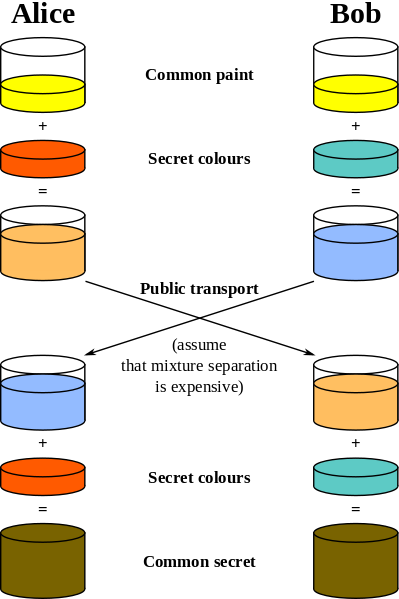
\includegraphics{res/Diffie-Hellman_Key_Exchange.png}

%%%%%%%%%%%%%%%%%%%%%%%%%%%%%%%%%%%%%%%%%%%%%%%%%%%%%%%%%%%%%%%%%%%%%
%
%	Malleable Encryption
%
%%%%%%%%%%%%%%%%%%%%%%%%%%%%%%%%%%%%%%%%%%%%%%%%%%%%%%%%%%%%%%%%%%%%%

\pagebreak
\vspace*{\fill}
\begin{center}
\section{Malleable Encryption}
A cryptographic algorithm is considered to be \textit{malleable}, if an encrypted cipher text of message \textit{m}, 
can be converted into another cipher text, which can be decrypted with known function \textit{f(m)}, without 
prior knowledge of \textit{m}. Malleability does not refer to ability to read the encrypted message. \\
\end{center}
\vspace*{\fill}
\pagebreak


\subsection{Malleability in Encryption}


Generally, \textit{Malleability} is an undesirable property for any crypto system. But for certain special 
cases, like \textit{Homomorphic Encryption,} [: form of encryption which allows specific type of operations on
cipher text, to generate a cipher text, which when decrypted matches to the operations performed on plain 
text.]

\subsubsection{RSA Example}
To demonstrate malleability, we can consider RSA encryption scheme.

\bigskip

RSA Encryption scheme for encrypting a message \textit{m}, using the public key pair (e,n), can be expressed 
as,
\bigskip

\begin{center}
$E(m) = (m)^e \bmod n$
\end{center}

Given the above parameters, except \textit{m}, it is still possible to construct encryption of message \textit{E(mt)} as below.
\bigskip

\begin{center}
$ E(m).t^e \bmod n = ((m)^e \bmod n).(t^e \bmod n)$
$                       = ((m.t)^e \bmod n)$
$                       = E(mt)$
\end{center}





%%%%%%%%%%%%%%%%%%%%%%%%%%%%%%%%%%%%%%%%%%%%%%%%%%%%%%%%%%%%%%%%%%%%%
%
%	ElGamal Encryption
%
%%%%%%%%%%%%%%%%%%%%%%%%%%%%%%%%%%%%%%%%%%%%%%%%%%%%%%%%%%%%%%%%%%%%%

\pagebreak
\vspace*{\fill}
\begin{center}
\section{ElGamal Encryption}
This section is study notes on ElGamal Encryption Scheme, a \textit{asymmetric key encryption} algorithm,
based on \textit{Diffie-Helman Key exchange}, proposed by \textit{Taher Elgamal}, in 1985.
\end{center}
ElGamal encryption can be defined over any cyclic group G. \\
Its security depends upon the \textbf{difficulty of computing discrete logarithms.}
\vspace*{\fill}
\pagebreak

\subsection{Algorithm}
ElGamal encryption consists of three components: 
\begin{itemize}

\item Key generator,
\item Encryption algorithm,
\item Decryption algorithm.
\end{itemize}

\subsubsection{Key generation}
\begin{itemize}
\item Define \textbf{cyclic group}  \(G\), of order \(q\) with generator \(g\).
\item Choose a random number \(x\) from \{1,..\(q\)-1\}
\item Compute \(p\) = $g^{x}$\\
\textbf{\item The tuple (\(G\), \(q\),\(g\),\(p\)) is public key.
\item \(x\) is the private key}
\end{itemize}

\subsubsection{Encryption}
\begin{itemize}
\item Randomly choose \(y\) from \{1,..\(q\)-1\}
\item Calculate shared secret $s = p^y$
\item Covert message \(m\) into \(m\)' of \(G\)
\item Calculate \(c_{1}\) = $g^y$
\item Calculate \(c_{2}\) = \(m\)'.\(s\) 
\item Calculate $(c_{1},c_{2})=(g^y, m'\cdot p^y)=(g^y, m'\cdot(g^x)^y)$ \\
\item If \(m\) is known, \(m\)' can be calculated from which, $p^y$ can be calculated
\end{itemize}

\subsubsection{Decryption}
\begin{itemize}
\item calculates the shared secret $s=c_1^x\,$
\item computes $m'=c_2 \cdot s^{-1}\,$
\item $c_2 \cdot s^{-1} = m'\cdot p^y \cdot (g^{xy})^{-1} = m'\cdot g^{xy} \cdot g^{-xy} = m'.$
\end{itemize}

%\begin{msc}{Elgamal}
%
%\declinst{usr}{User}{}
%\declinst{m1}{Machine 1}{control}
%\declinst{m2}{Machine 2}{drill}
%\declinst{m3}{Machine 3}{test}
%
%\mess{startm1}{usr}{m1}
%\nextlevel
%\mess{startm2}{m1}{m2}
%\nextlevel
%\mess{continue}{m2}{m3}
%\mess{log}{m1}{envleft}
%\nextlevel
%\mess{output}{m3}{usr}[2]
%\nextlevel
%\mess{free}{m1}{usr}
%\nextlevel
%
%\end{msc}

\subsection{Security of ElGamal Encryption}
\begin{itemize}

\item The security of the ElGamal scheme depends on the properties of the underlying group G as well as any padding scheme used on the messages.
\item If the \textit{computational Diffie–Hellman assumption} (CDH) holds in the underlying cyclic group G, then the encryption function is one-way.
\item If the \textit{decisional Diffie–Hellman assumption} (DDH) holds in G, then ElGamal achieves \textit{semantic security}.
\item Elgamal Encryption is \textit{\textbf{Unconditionally Malleable}}
\item Hence it is \textit{\textbf{Not secure under Chosen Ciphertext attack} (CCA)}
\item i.e. If $(c_1, c_2)$ are given for any message \(m\), its easy to calculate, $(c_1, 2c_2)$ in order to 
decrypt message $2m$
\item To achieve CCA security, appropriate padding scheme should be used.
\end{itemize}








%%%%%%%%%%%%%%%%%%%%%%%%%%%%%%%%%%%%%%%%%%%%%%%%%%%%%%%%%%%%%%%%%%%%%
%
%	Certificate Less Key Exchange, In Presence of a Strong Adversary
%
%%%%%%%%%%%%%%%%%%%%%%%%%%%%%%%%%%%%%%%%%%%%%%%%%%%%%%%%%%%%%%%%%%%%%


\pagebreak
\vspace*{\fill}
\begin{center}
\section{Certificate Less Key Exchange, In Presence of a Strong Adversary}
Exchanging two public key, over an insecure channel or without any presence of earlier shared secret, 
always needs a certificate to be issued by a \textit{Trusted Third party}, aka, \textit{Certifying Authority}.
But this is not always possible, especially in \textit{Ad hoc} networks. We propose a solution to such a 
scenario, to exchange the key, over an insecure channel, in presence of such the strong adversary, who has 
access to all of the messages transmitted over the channel and who can modify the message if he wishes.
\end{center}
\vspace*{\fill}
\pagebreak


%%%%%%%%%%%%%%%%%%%%%%%%%%%%%%%%%%%%%%%%%%%%%%%%%%%%%%%%%%%%%%%%%%%%%
%
%	Zero Knowledge Proof
%
%%%%%%%%%%%%%%%%%%%%%%%%%%%%%%%%%%%%%%%%%%%%%%%%%%%%%%%%%%%%%%%%%%%%%

\pagebreak
\vspace*{\fill}
\begin{center}
\section{Zero Knowledge Proof}
This section is study notes on Zero Knowledge Proof Protocol.
\end{center}
\vspace*{\fill}
\pagebreak

\subsection{Introduction}
\begin{itemize}
\item A Zero-knowledge proof or Zero-knowledge protocol is a protocol used in cryptography. 
\item The are two parties communicating. 
\item The task of one party is to convince the other that it knows some secret, without revealing the secret.
\item The prover of the statement is called as Peggy 
\item The verifier of the statement is Victor 
\item It requires some secret information on the part of the prover
\item The definition implies that the verifier will not be able to prove the statement to anyone else
\item An real-world example of such a protocol is the Feige-Fiat-Shamir Identification Scheme.
\end{itemize}

\subsection{Story}
\subsubsection{Epilogue}
\begin{itemize}
\item Peggy has uncovered the secret word used to open a magic door in a cave
\item The cave is shaped like a circle, with entrance on one side \& magic door blocking the opposite side.
\item Victor says he'll pay her for the secret, but not until he's sure that she really knows it.
\item Peggy says she'll tell him the secret, but not until she receives the money.
\item They devise a scheme by which Peggy can prove that she knows the word without telling it to Victor.
\end{itemize}

\subsubsection{The Story}
\begin{itemize}
\item First, Victor waits outside the cave as Peggy goes in.
\item They label the left and right paths from the entrance A and B.
\item Peggy randomly takes either path A or B.
\item Then, Victor enters the cave and shouts the name of the path he wants her to use to return
\item Providing she really does know the magic word, this is easy:
\item she opens the door, if necessary, and returns along the desired path.
\item Note that Victor does not know which path she has gone down.
\item The correctness can only be 50\% in this scheme
\item If they were to repeat this trick many times, say 20 times in a row, 
\item $=>$ her chance of successfully anticipating all of Victor's requests would become very small.
\item For this reason, if Peggy reliably appears at the exit Victor names, he can conclude that \textbf{\textit{\color{blue} she is very likely}} \color{black} to know the secret word.	
\end{itemize}

\subsection{Properties of ZKP}
A zero-knowledge proof must satisfy three properties:
\begin{enumerate}
\item Completeness
\item Soundness
\item Zero Knowledge
\end{enumerate}
\paragraph{Completeness} : if the statement is true, the honest verifier (that is, one following the protocol properly) will be convinced of this fact by an honest prover.
\paragraph{Soundness} : if the statement is false, no cheating prover can convince the honest verifier that it is true, except with some small probability.
\paragraph{Zero Knowledge} : The verifier should know only the fact that prover can prove. 

\begin{itemize}
\item The first two of these are properties of more general interactive proof systems. 
\item The third is what makes the proof zero-knowledge.
\end{itemize}

\subsection{The soundness error}
The small probability that prover can use to cheat verifier is called as \textbf{The soundness error}.
ZKP are probabilistic "proofs" rather than deterministic proofs.







%%%%%%%%%%%%%%%%%%%%%%%%%%%%%%%%%%%%%%%%%%%%%%%%%%%%%%%%%%%%%%%%%%%%%
%
%	English Vocabulary
%
%%%%%%%%%%%%%%%%%%%%%%%%%%%%%%%%%%%%%%%%%%%%%%%%%%%%%%%%%%%%%%%%%%%%%

\pagebreak
\vspace*{\fill}
\begin{center}
\section{English Vocabulary}
\end{center}
\vspace*{\fill}
\pagebreak

This is study notes on The Structure of English Words (LING150) course from http://darkwing.uoregon.edu/~l150web/index.html
\subsection{Course Organization}
\begin{itemize}
\item \textbf{Unit 1:} Basic Word Analysis
\begin{itemize}
\item Historical sources of English words
\item Basic principles of word analysis (morphology)
\end{itemize}
\item \textbf{Unit 2:} Intermediate Word Analysis and Basic Phonetics
\begin{itemize}
\item Alternations in morpheme forms (allomorphy)
\item Basic principles of English sounds (phonetics)
\end{itemize}
\item \textbf{Unit 3:} Advanced Word Analysis and Semantic Change
\begin{itemize}
\item More alternations in morpheme forms (allomorphy rules)
\item Historical changes of meanings (semantic change)
\end{itemize}
\item \textbf{Unit 4:} - The Origins and History of English
\begin{itemize}
\item Pre-history of English and Indo-European languages
\item English history
\end{itemize}
\end{itemize}

\subsection{Introduction to English vocabulary}
\subsubsection{Sources of English words}
\begin{center}
\Tree [.Engligh\ Words [.Native\ Words ] [.Borrowed\ Words [.Classic\ Languages [.Greek ] [.Latin ]] [.Exotic\ Languages ] ]]
\end{center}


The native words are words which are used in evryday conversations. The native words falls into follwoing categories. \\
\\
\begin{tabular}{| l | c | }
	\hline	
		\textbf{Type} & \textbf{Example} \\
		\hline 		\hline
		Body Parts & Foot, mouth, hand, leg \\ \hline
		Family Relationships / Kinship terms & Father, mother, brother, sister \\ \hline
		Everyday, Natural objects &  rock, house, hill \\ \hline
		Physical Acts &  think, drive, ride \\ \hline
		Physical charactrestics  & red, cold, young \\ \hline 
\end{tabular}
\subsubsection{Learning Model}
Learning new words and improving new vocabulary can be carried out by the following ways.
\begin{itemize}
\item Absorption
\item Memorization
\item Analysis
\end{itemize}

\subsection{Analyzing words}
\subsubsection{Morphemes}
Word analysis involves breaking a word into its morphemes. Literally morphemes means \textbf{\textit{an element in a system of forms.}}\\
In linugustics, it is defined as 
\begin{addmargin}[3em]{2em}% 1em left, 2em right
"The smallest \textbf{\textit{form}} which is paired with a particular \textbf{\textit{meaning}}"
\end{addmargin} 
From Dictionary: \textbf{\textit{morpheme}}, noun, very rare\\
\begin{addmargin}[3em]{2em}% 1em left, 2em right
	Minimal meaningful language unit;\\ 
	It cannot be divided into smaller meaningful units;
\end{addmargin}

\subsubsection{Characteristics of morphemes}
Morphemes have four defining characteristics:
\begin{itemize}
\item \color{blue} They cannot be subdivided.
\color{black} \item \color{blue} They add meaning to a word.
\color{black} \item \color{blue} They can appear in many different words.
\color{black} \item \color{blue} They can have any number of syllables.
\end{itemize}
\color{black}

\subsubsection{Problems with morphemes}
There is no one-to-one mapping between \textit{FORM} $\leftrightarrow$ \textit{MEANING}
\begin{itemize}
\item One form, two (or more) meanings.
	\begin{addmargin}[3em]{2em}% 1em left, 2em right
	\color{red}\textbf{in}- \color{blue}'\textit{not}' \color{black}in words like \color{red}\textbf{in}\color{black}capable and \color{red}\textbf{in}\color{black}sufficient, \& \\
	\color{red}\textbf{in}- \color{blue}'\textit{into, within}', \color{black}as in \color{red}\textbf{in}\color{black}vade and \color{red}\textbf{in}\color{black}clude.
	\end{addmargin}

\item Two (or more) forms, one meaning.
\begin{itemize}
\item Two (or more) forms, one meaning = two morphemes
	\begin{addmargin}[3em]{2em}% 1em left, 2em right
	\color{red}\textbf{andr}- \color{blue}'\textit{man,male}' \color{black}in words like \color{red}\textbf{and}\color{black}roid \& \\
	\color{red}\textbf{vir}- \color{blue}'\textit{man,male}', \color{black}as in \color{red}\textbf{vir}\color{black}ile
	\end{addmargin}

\item Two (or more) forms, one meaning = one morpheme
	\begin{addmargin}[3em]{2em}% 1em left, 2em right
		\color{red} \textbf{pan-} \color{black} and \color{red} \textbf{pant-} \color{black}, which are different forms of a Greek morpheme meaning \color{blue}'all,overall'. 
	\end{addmargin}

\end{itemize}
\end{itemize}
The alternate forms of a single morpheme are called \color{blue}\textbf{allomorphs},\color{black} literally 'other forms.' 

\subsubsection{How to analyze words}
\begin{itemize}
\item Only Words borrowed from Classic languages like Greek and Latin can be analyzed
\item Native words or words borrowed from exotice languages can not be analyzed
\end{itemize}
There are four steps as following in analyzing a word
\begin{itemize}
\item Parse : Divide it into its morpheme
\item Gloss : Give the meaning for a morpheme
\item Give a literal meaning :  Use the meanings from the glosses to construct a literal meaning
\item Give a dictionary definition : Extended literal meaning metaphorically to arrive at the actual meaning.
\end{itemize}

Example :
	\begin{addmargin}[3em]{2em}% 1em left, 2em right
	\begin{itemize}
	\item \color{red} \textbf{repellent} \color{black} 
	\item re-  /  pel  /  (l)  /  -ent
	\item 'again, back' / 'push' / (l) / A, N
	\item 'something which pushes back' / (l) /A,N
	\end{itemize}
	\end{addmargin}
	
'A, N.' : The letters stand for 'ADJECTIVE, NOUN'

\subsection{Words - their construction and use}
\begin{enumerate}
\item How words are constructed
\begin{enumerate}
\item Types of Roots
\item Types of Affixes
\end{enumerate}
\item How words are used - NOUNS, VERBS and ADJECTIVES
\end{enumerate}

\subsubsection{How words are constructed}
\begin{center}
\Tree [.Morphemes [.ROOTS [.Free\ Root ] [.Bounded\ Root ]] [.AFFIXES [.Prefixes ] [.Suffixes ] ]]
\end{center}
\paragraph{Roots}
\begin{itemize}
\item Roots usually have a rather specific meaning
\item This meaning tends to be relatively constant across all the words that use the root. 
\item Roots also contribute the greatest conceptual content to the overall meaning of the word.
\item Every word has at the least one root. 
\item Roots have freer distribution; that is, they can occur almost anywhere in a word
\item Two ore more roots combine to form Compound words.
\item Compound words may or may not have affixes.
\end{itemize}

\subparagraph{Free Roots}
\begin{itemize}
\item Free Roots are roots that can occur alone as whole words
\item They can stand alone as single words.
\item Free roots can also be combined with other roots or affixes to form more complex words
\end{itemize}

\subparagraph{Bounded Roots}
\begin{itemize}
\item Bound Roots can never occur alone as whole words.
\item They cannot stand alone; 
\item They must occur in combination with other morphemes
\item Almost all the Latin and Greek roots we are studying are bound roots
\end{itemize}

\paragraph{Affixes}
\begin{itemize}
\item Affixes are morphemes which attach to roots or a combination of roots and other affixes. 
\item Their main use is to modify the meaning conveyed by the root or roots.
\item Affixes by definition are always bound or affixed to a root. 
\item They are divided into two different types depending on where they attach to the root.
\item \color{blue}Prefixes \color{black}occur before a root (although several prefixes can be strung together before a single root).
\item \color{blue}Suffixes \color{black}occur after a root (although multiple suffixes can occur at the ends of words).
\end{itemize}

\subsection{Suffixes and Prefixes}
\begin{enumerate}
\item Suffixes 
\begin{enumerate}
\item Inflectional suffixes
\begin{itemize}
\item Add only grammatical information
\item Never change the part of speech
\end{itemize}
\begin{tabular}{| l | c | }
	\hline	
		\textbf{Rule} & \textbf{Explanation} \\
		\hline
		\hline
			\color{red} -s \color{black} 'plural' &  The two girl\color{red}s \color{black}had eaten dinner  \\ \hline
			\color{red} -'s \color{black}'possessive' & The cat\color{red}'s \color{black}tail was twitching   \\ \hline
			\color{red} -ed \color{black}'past tense' & The blackest dog never bark\color{red}ed  \\ \hline
			\color{red} -s \color{black}'3rd person present tense' & The smaller dog bark\color{red}s \color{black}a lot  \\ \hline
			\color{red} -ing \color{black}'present participle' & The cat's tail was twitch\color{red}ing  \\ \hline
			\color{red} -en \color{black}'past participle' &  The two girls had eat\color{red}en \color{black}dinner  \\ \hline
			\color{red} -er \color{black}'comparative' & The small\color{red}er \color{black}dog barks a lot  \\ \hline
			\color{red} -est \color{black}'superlative' &  The black\color{red}est \color{black}dog never barked  \\ \hline
\end{tabular}
\item Derivational suffixes
\begin{itemize}
\item Make a new word with a new meaning
\item Usually change the part of speech
\end{itemize}
\item Meanings of Derivational Suffixes
\end{enumerate}

\item Prefixes
\begin{enumerate} 
\item Spatial Prefixes
\begin{itemize}
\item The largest group of prefixes denote relationships that occur in space.
\end{itemize}
\item Non-Spatial Prefixes
\begin{itemize}
\item Comparative relations
\item Quantity and Size
\item Negative Prefixes
\item Intensive prefixes
\end{itemize}
\end{enumerate}
\end{enumerate}




%%%%%%%%%%%%%%%%%%%%%%%%%%%%%%%%%%%%%%%%%%%%%%%%%%%%%%%%%%%%%%%%%%%%%
%
%	Number-Theoretic Reference Problems
%
%%%%%%%%%%%%%%%%%%%%%%%%%%%%%%%%%%%%%%%%%%%%%%%%%%%%%%%%%%%%%%%%%%%%%

\pagebreak
\vspace*{\fill}
\begin{center}
\section{Number-Theoretic Reference Problems}
\end{center}
\vspace*{\fill}
\pagebreak
\subsection{Introduction}
\begin{itemize}
\item Security of many public-key cryptosystems dependent on intractability of the computational problems.
\item A problem is tractable if its possible to solve in polynomial time.
\item Problem \textit{A} can be said as reducable to Problem \textit{B}, if A can be solved by employing B and other finite operations $\xi.$
\item If A $\leq_{p}$ B, (i.e, A is reducable to B), then A is \textit{Computationaly Equivalent} to B, written as A $\equiv_{p}$ B
\item If  A $\equiv_{p}$ B, then both are tractabe or intractable.
\end{itemize} 

\subsection{Integer Factorization Problem}
\begin{itemize}
\item Given a positive integer $\textit{n}$, find its prime factors;
\item Write n $\mid$ $n = p_{1}^{e_{1}}p_{2}^{e_{2}}...p_{k}^{e_{k}}$, where $p_{i}$ are pairwise primes and $e_{i} \geq 1.$
\item  A set of integers is said to be pairwise coprime if a and b are coprime for every pair (a, b) of different integers in it.
\end{itemize}







%%%%%%%%%%%%%%%%%%%%%%%%%%%%%%%%%%%%%%%%%%%%%%%%%%%%%%%%%%%%%%%%%%%%%
%
%	Cryptographic Primitives
%
%%%%%%%%%%%%%%%%%%%%%%%%%%%%%%%%%%%%%%%%%%%%%%%%%%%%%%%%%%%%%%%%%%%%%
\section{Cryptographic Primitives}
\subsection{Introduction}
\paragraph{A symmetric or private-key cipher} is one in which knowledge of the encryption key is explicitly or implicitly equivalent to knowing the decryption key.
\paragraph{An asymmetric or public-key cipher} is one in which the encryption key is effectively public knowledge, without giving any useful information about the decryption key.

\paragraph{trapdoor } is a computation which runs much more easily in one direction than back.

\paragraph{Example : }Multiplication of large integers is easy, while factoring of large integers is difficult.\\
Merely testing large numbers for primality is easy.

\subsection{RSA Cipher}
\begin{enumerate}
\item Generate two primes, p and q, such that, atleast $>2^{512}$ or preferably $>2^{1024}$
\item Compute \textbf{RSA Modulus, n =p.q}
\item Choose encryption exponent, \textbf{e} $> 2$, \textbf{randomly.} \\
Often, its \textbf{Fermats number} [A positive integer, of form, \textbf{$F_{n}=2^{2^{n}} + 1$} ]\\
\begin{center}
e = $2^{16} +1 = 65537$
\end{center}
\item Make \textbf{\textit{n}} and \textbf{\textit{e}} public
\item Compute decryption exponent, such that,\\
\begin{center}
$e.d = 1 \hspace{5pt} mod \hspace{5pt} (p-1)(q-1)$
\end{center}
\item Encryption : $E_{n,e}(x) = x ^{e} \hspace{5pt} \% \hspace{5pt}n \Rightarrow y $
\item Decryption : $D_{n,d}(y) = y ^{d} \hspace{5pt} \% \hspace{5pt}n \Rightarrow x $
\end{enumerate}







%%%%%%%%%%%%%%%%%%%%%%%%%%%%%%%%%%%%%%%%%%%%%%%%%%%%%%%%%%%%%%%%%%%%%
%
%	Logarithms
%
%%%%%%%%%%%%%%%%%%%%%%%%%%%%%%%%%%%%%%%%%%%%%%%%%%%%%%%%%%%%%%%%%%%%%
\pagebreak
\section{Logarithms}
\subsection{Logarithm definition}

If, a number \textit{b} is raised to a power \textit{x}, such that,\\
\begin{center}	$b^{x} = y$		\end{center}

Then the base b logarithm of x is equal to y:

\begin{center} 	log$_{b}(x) = y$	\end{center}

Then, we can conjure logarithms as the inverse of exponentiation, like
\begin{center}	$b^{y} = x $		\end{center}
\paragraph{Example :\\}
\begin{center}
log$_{2}(32) = 5$	$\Rightarrow 2^{5} = 32 $
\\log$_{2}(16) = 4$ $\Rightarrow 2^{4} = 16 $
\\log$_{2}(8) = 3$ $\Rightarrow 2^{3} = 8 $
\end{center}

\subsection{Logarithms Rules}
\begin{tabular}{| l | c | }
	\hline	
		\textbf{Rule} & \textbf{Explanation} \\
		\hline
		\hline
		Logarithm product rule 		& $log_{b}(x . y) = log_{b}(x) + log_{b}(y)$ \\ \hline
		Logarithm quotient rule 		& $log_{b}(x / y) = log_{b}(x) - log_{b}(y)$ \\ \hline
		Logarithm power rule			& $log_{b}(x ^{y}) = y . log_{b}(x)$  \\ \hline
		Logarithm base switch rule 	& $log_{b}(c) = 1 / log_{c}(b)$	\\ \hline
		Logarithm base change rule 	& $log_{b}(x) = log_{c}(x) / log_{c}(b)$	\\ \hline
		Derivative of logarithm		& $f(x) = log_{b}(x) \Rightarrow f^{'}(x) = 1 / ( x ln(b))$ \\ \hline
		Integral of logarithm		& $\int log_{b}(x) dx = x . ( log_{b}(x) - 1 / ln(b) ) + C$  \\ \hline
		Logarithm of negative number & $log_{b}(x)$ is undefined when $x \le 0$   \\ \hline
		Logarithm of 0				& $log_{b}(0)$ is undefined \\ & $\lim_{x\to 0^+}\textup{log}_b(x)=-\infty$   \\ \hline
		Logarithm of 1				& $log_{b}(1) = 0$  \\ \hline
		Logarithm of the base		& $log_{b}(b) = 1$  \\ \hline
\end{tabular}





%%%%%%%%%%%%%%%%%%%%%%%%%%%%%%%%%%%%%%%%%%%%%%%%%%%%%%%%%%%%%%%%%%%%%
%
%	English Syllables
%
%%%%%%%%%%%%%%%%%%%%%%%%%%%%%%%%%%%%%%%%%%%%%%%%%%%%%%%%%%%%%%%%%%%%%
\section{English Syllables}
\paragraph{Divide words based on the number of vowels: } The number of syllables in a word coincide with the number of vowel sounds you hear when speaking the word.  \\

Example : B\underline{a} $\mid n\underline{a} \mid$ n\underline{a}

\paragraph{Vowels:} 'a,' 'e,' 'i,' 'o,' 'u' and 'y' are considered as vowels, when found in the middle or at the end of a word.

\subparagraph{Subtract 1 for each silent vowel in the word:} Example : 'came' and 'gone,' 'E' is the most common silent vowel.

\subparagraph{Consider words ending in 'le' as a vowel:} Divide the word before the consonant right before the 'le'. \\
Example : Little would be divided lit/tle; fumble as fum/ble; able as a/ble.

\subparagraph{Count diphthongs as 1 syllable instead of 2 : } diphthongs are two vowels, combined giving one syllable. Example : Words like 'h\underline{au}l,' 'm\underline{oo}n,' and 'c\underline{oi}l' are diphthongs.

\subparagraph{Split words between consonants, surrounded by vowels.} Example :  hap/py, din/ner, bas/ket, un/der. 

\subparagraph{Find syllables by splitting a word before a single consonant. Examples are: au/tumn, o/pen, de/tail:}

\subparagraph{Mark prefixes and suffixes as syllabels: }



%%%%%%%%%%%%%%%%%%%%%%%%%%%%%%%%%%%%%%%%%%%%%%%%%%%%%%%%%%%%%%%%%%%%%
%
%	Group
%
%%%%%%%%%%%%%%%%%%%%%%%%%%%%%%%%%%%%%%%%%%%%%%%%%%%%%%%%%%%%%%%%%%%%%
\pagebreak
\section{Group}

A group G is a finite or infinite set of elements together with a binary operation (called the group operation) that together satisfy the four fundamental properties of \#1 closure, \#2 associativity, \#3 the identity property, and \#4 the inverse property. 

\paragraph{1. Closure:} If A and B are two elements in G, then the product AB is also in G.

\paragraph{2. Associativity:} The defined multiplication is associative, i.e., for all A,B,C in G, (AB)C=A(BC).

\paragraph{3. Identity:} There is an identity element I (a.k.a. 1, E, or e) such that IA=AI=A for every element A in G.

\paragraph{4. Inverse:} There must be an inverse (a.k.a. reciprocal) of each element. Therefore, for each element A of G, the set contains an element B=A\^(-1) such that AA\^(-1)=A\^(-1)A=I.

\paragraph{Group Theory:} Study of groups.

\paragraph{Finite Group:} The group has a finite number of elements.

\paragraph{Subgroup:} A subset of group, which is \textit{closed} under \textit{group operation} is called as subgroup.

\paragraph{Cyclic Group:} Cyclic group is a group, that is generated by a single element. That is,
\begin{itemize}
\item It consists of a set of elements, with single invertible associative operation and
\item a element g, such that, every other element in the group can be obtained by applying the group operation or its inverse to g.
\end{itemize}

Cyclic group is closed under addition, associative and has unique inverse.

\paragraph{Homomorphism:} A map between two groups, which preserve identity and group operation is called Homomorphism.

\paragraph{Isomorphism:} If a homomorphism has an inverse which is also an homomorphism, this is called as \textit{isomorphism} and the two group is said to be isomorphic.

%%%%%%%%%%%%%%%%%%%%%%%%%%%%%%%%%%%%%%%%%%%%%%%%%%%%%%%%%%%%%%%%%%%%%
%
%	Android Services
%
%%%%%%%%%%%%%%%%%%%%%%%%%%%%%%%%%%%%%%%%%%%%%%%%%%%%%%%%%%%%%%%%%%%%%


\pagebreak
\section{Android Services}
\label{Android Services}

We will see, 
\begin{enumerate}
\item What is a Service?
\item Service Life-cycle
\item Permissions
\item Process Life-cycle
\item Local Service Sample
\item Remote Messenger Service Sample
\end{enumerate}

\subsection{Introduction}
A Service is an application component, representing either 
\begin{itemize}
\item{an application's desire to perform a longer-running operation while not interacting with the user. \textit{This corresponds to calls to \textbf{Context.startService()}}}
\item{to supply functionality for other applications to use. \textit{This corresponds to calls to \textbf{Context.bindService()}}}
\end{itemize} 
Service is 
\begin{itemize}
\item Not a seperate process
\item Not a seperate thread
\end{itemize}
Each service class must have a corresponding $<$service$>$ declaration in its package's \textit{\textbf{AndroidManifest.xml.}} \\
Services can be started with \textbf{\textit{Context.startService()}} and \textbf{\textit{Context.bindService().}}\\


\subsection{Service Lifecycle}
 If someone calls \textit{Context.startService()} $\longrightarrow$ \textit{onCreate()} $\longrightarrow$ \\ \textit{onStartCommand(Intent, int, int) } $\longrightarrow$  run until \textit{Context.stopService()} or \textit{stopSelf()} is called

\textit{START\_STICKY} is used for services that are explicitly started and stopped as needed. \\
\textit{START\_NOT\_STICKY} or \textit{START\_REDELIVER\_INTENT} are used for services that should only remain running while processing any commands sent to them.\\
\textit{onDestroy()} method is called and the service is effectively terminated.

\subsection{Permissions}
Global access to a service can be enforced when it is declared in its manifest's $<$service$>$ tag. 
By doing so, other applications will need to declare a corresponding $<$uses-permission$>$ element in their own manifest to be able to start, stop, or bind to the service.\\
This can be bypassed by using \textit{Intent.FLAG\_GRANT\_READ\_URI\_PERMISSION} and/or \textit{Intent.FLAG\_GRANT\_WRITE\_URI\_PERMISSION }on the Intent, when using \textit{Context.startService(Intent)}.
\pagebreak


%%%%%%%%%%%%%%%%%%%%%%%%%%%%%%%%%%%%%%%%%%%%%%%%%%%%%%%%%%%%%%%%%%%%%
%
%	Two step verification
%
%%%%%%%%%%%%%%%%%%%%%%%%%%%%%%%%%%%%%%%%%%%%%%%%%%%%%%%%%%%%%%%%%%%%%
\section{Two step verification}
\subsection{Factors of Authentication}
\begin{tabular}{| l | c | r | p{0.000002}}
	\hline	
		Factor & Explanation & Example\\
		\hline
		\hline
		Ownership factor & Something that user has & ID Card, A hardware, Token \\ \hline
		Knowledge factor & Something that user knows & Password, PIN \\	\hline
		Inherence factor & Something that is inhere to user & Biometrics like fingerprint, retina etc\\
	\hline
\end{tabular}
\subsection{Two step verification}
For a secured and positive authentication, atleast there should be two or all three factors involve in authentication.
\paragraph{Single Sign On} A method to authenticate in a system which has multiple secured, independent systems. By this Single Sig On, a user logins in and autheticates one system and gains acess to all the systems.
\pagebreak

%%%%%%%%%%%%%%%%%%%%%%%%%%%%%%%%%%%%%%%%%%%%%%%%%%%%%%%%%%%%%%%%%%%%%
%
%	Newline representation
%
%%%%%%%%%%%%%%%%%%%%%%%%%%%%%%%%%%%%%%%%%%%%%%%%%%%%%%%%%%%%%%%%%%%%%
\section{Newline representation}

\paragraph{Carriage Return [CR] : } Reset typewriters horizontal position to the far left.
\paragraph{Line Feed [LF] : } Advance the paper by one line.
\\
\\
\textit{ASCII }Based systems 

A type writer typically needs both.
Windows uses CR+LF.
Linux uses only LF.
MAC OS, prior to OS-X used CR alone.
\\

IBM Pc's based on EBCDIC uses a special character called as \textit{Newline \textbf{[NL]}}
\pagebreak



%%%%%%%%%%%%%%%%%%%%%%%%%%%%%%%%%%%%%%%%%%%%%%%%%%%%%%%%%%%%%%%%%%%%%
%
%	Turing Machine
%
%%%%%%%%%%%%%%%%%%%%%%%%%%%%%%%%%%%%%%%%%%%%%%%%%%%%%%%%%%%%%%%%%%%%%
\section{Turing Machine}

A Turing machine can be thought of as a primitive, abstract computer. Alan Turing, who was a British mathematician and cryptographer, invented the Turing machine as a tool for studying the computability of mathematical functions. Turing's hypothesis (also known has Church's thesis) is a widely held belief that a function is computable if and only if it can be computed by a Turing machine. This implies that Turing machines can solve any problem that a modern computer program can solve. There are problems that can not be solved by a Turing machine (e.g., the halting problem); thus, these problems can not be solved by a modern computer program.

\subsection{Components of a Turing Machine}
A Turing machine has
\begin{itemize}
\item an infinite tape that consists of adjacent cells (or squares). 
\item On each cell is written a symbol. The symbols that are allowed on the tape are finite in number and include the blank symbol. 
\item Each Turing machine has it's own alphabet (i.e., finite set of symbols), which determines the symbols that are allowed on the tape.
\item a tape head that is positioned over a cell on the tape. This tape head is able to read a symbol from a cell and write a new symbol onto a cell. 
\item The tape head can also move to an adjacent cell (either to the left or to the right).
\item A Turing machine has a finite number of states, and, at any point in time, a Turing machine is in one of these states. 
\item A Turing machine begins its operation in the start state. 
\item A Turing machine halts when it moves into one of the halt states.
\end{itemize} 
\pagebreak
\subsection{Opeartion of a Turing Machine}
\begin{enumerate}
\item The Turing machine reads the tape symbol that is under the Turing machine's tape head. This symbol is referred to as the current symbol.
\item The Turing machine uses its transition function to map the following: 
\begin{center}
\{the current state and current symbol\} =  \{the next state, the next symbol and the movement for the tape head.\}
\end{center}
\item The Turing machine changes its state to the next state, which was returned by the transition function.
\item The Turing machine overwrites the current symbol on the tape with the next symbol, which was returned by the transition function.
\item The Turing machine moves its tape head one symbol to the left or to the right, or does not move the tape head, depending on the value of the 'movement' that is returned by the transition function.
\item If the Turing machine's state is a halt state, then the Turing machine halts. Otherwise, repeat sub-step \#1.
\end{enumerate}


%%%%%%%%%%%%%%%%%%%%%%%%%%%%%%%%%%%%%%%%%%%%%%%%%%%%%%%%%%%%%%%%%%%%%
%
%	NP Complete
%
%%%%%%%%%%%%%%%%%%%%%%%%%%%%%%%%%%%%%%%%%%%%%%%%%%%%%%%%%%%%%%%%%%%%%
\section{NP Complete}
Decision problem :
Any problem with an answer, YES or NO.

\paragraph{P :} A decision problem that can be solved in polynomial time. That is, given an instance of the problem, the answer yes or no can be decided in polynomial time.

\subparagraph{\textit{Example : }} Given a graph connected G, can its vertices be colored using two colors so that no edge is monochromatic. Algorithm: start with an arbitrary vertex, color it red and all of its neighbors blue and continue. Stop when you run our of vertices or you are forced to make an edge have both of its endpoints be the same color.

\paragraph{NP :} A decision problem where instances of the problem for which the answer is yes have proofs that can be verified in polynomial time. This means that if someone gives us an instance of the problem and a certificate (sometimes called a witness) to the answer being yes, we can check that it is correct in polynomial time.

\subparagraph{\textit{Example:}} Integer factorization is NP. This is the problem that given integers n and m, is there an integer f with 1 < f < m such that f divides n (f is a small factor of n)? This is a decision problem because the answers are yes or no. If someone hands us an instance of the problem (so they hand us integers n and m) and an integer f with 1 < f < m and claim that f is a factor of n(the certificate) we can check the answer in polynomial time by performing the division n / f.

\paragraph{NP-complete :} An NP problem X for which it is possible to reduce any other NP problem Y to X in polynomial time. Intuitively this means that we can solve Y quickly if we know how to solve X quickly. Precisely, Y is reducible to X if there is a polynomial time algorithm f to transform instances x of X to instances y = f(x) of Y in polynomial time with the property that the answer to x is yes if and only if the answer to f(x) is yes.

\subparagraph{\textit{Example:}} 3-SAT. This is the problem wherein we are given a conjunction of 3-clause disjunctions (i.e., statements of the form

(x\_v11 or x\_v21 or x\_v31) and 
(x\_v12 or x\_v22 or x\_v32) and 
...                       and 
(x\_v1n or x\_v2n or x\_v3n)
where each x\_vij is a boolean variable or the negation of a variable from a finite predefined list (x\_1, x\_2, ... x\_n). It can be shown that every NP problem can be reduced to 3-SAT. The proof of this is technical and requires use of the technical definition of NP (based on non-deterministic Turing machines and the like). This is known as Cook's theorem.

What makes NP-complete problems important is that if a deterministic polynomial time algorithm can be found to solve one of them, every NP problem is solvable in polynomial time (one problem to rule them all).

\paragraph{NP-hard :} Intuitively these are the problems that are even harder than the NP-complete problems. Note that NP-hard problems do not have to be in NP (they do not have to be decision problems). The precise definition here is that a problem X is NP-hard if there is an NP-complete problem Y such that Y is reducible to X in polynomial time. But since any NP-complete problem can be reduced to any other NP-complete problem in polynomial time, all NP-complete problems can be reduced to any NP-hard problem in polynomial time. Then if there is a solution to one NP-hard problem in polynomial time, there is a solution to all NP problems in polynomial time.

The halting problem is the classic NP-hard problem. This is the problem that given a program P and input I, will it halt? This is a decision problem but it is not in NP. It is clear that any NP-complete problem can be reduced to this one.

\paragraph{P = NP :} This the most famous problem in computer science, and one of the most important outstanding questions in the mathematical sciences. In fact, the Clay Institute is offering one million dollars for a solution to the problem (Stephen Cook's writeup on the Clay website is quite good). It's clear that P is a subset of NP. The open question is whether or not NP problems have deterministic polynomial time solutions. It is largely believed that they do not. Here is an outstanding recent article on the latest (and the importance) of the P = NP problem: The Status of the P versus NP problem.

The best book on the subject is Computers and Intractability by Garey and Johnson. My favourite NP-complete problem is the Minesweeper problem.
\bibliographystyle{abbrv}
\bibliography{main}

\end{document}
